%\VignetteIndexEntry{NanoStringDiff Vignette}
%\VignettePackage{NanoStringDiff}
%\VignetteKeyword{NanoString}
%\VignetteKeyword{Differential Expression}

\documentclass[12pt]{article}

\usepackage{float}
\usepackage{Sweave}

\usepackage{amssymb}


\RequirePackage{Bioconductor}
\AtBeginDocument{\bibliographystyle{unsrturl}}

\renewcommand{\baselinestretch}{1.3}






\author{Hong Wang$^{1}$, Chi Wang$^{2,3}$\footnote{to whom correspondence 
should be addressed} \\[1em] 
\small{$^{1}$Department of Statistics , University of Kentucky,Lexington, KY;}\\ 
\small{$^{2}$Markey Cancer Center, University of Kentucky, Lexington, KY ;}\\ 
\small{$^{3}$Department of Biostatistics, University of Kentucky, 
Lexington, KY;}\\ 
\small{\texttt{hong.wang@uky.edu}}}



\title{\textsf{\textbf{The NanoStringDiff package}}}

%\bibliographystyle{abbrv}

\begin{document}
\Sconcordance{concordance:NanoStringDiff.tex:NanoStringDiff.Rnw:%
1 88 1 1 2 1 0 6 1 3 0 1 2 71 1 1 2 4 0 1 2 5 1 1 2 1 0 1 1 3 0 1 2 2 1 %
1 2 1 0 1 1 10 0 1 2 1 1 1 2 1 0 1 1 8 0 1 1 16 0 1 2 9 1 1 2 1 0 7 1 1 %
3 2 0 1 2 1 0 1 1 15 0 1 1 9 0 1 1 12 0 1 2 26 1 1 2 1 0 3 1 15 0 1 2 7 %
1 1 2 4 0 1 2 3 1 1 2 1 0 1 1 6 0 1 1 6 0 1 1 7 0 1 2 2 1 1 2 1 0 1 1 %
11 0 1 1 33 0 1 2 19 1 1 2 1 0 5 1 1 3 2 0 1 2 1 0 1 1 15 0 1 1 18 0 1 %
2 3 1 1 2 1 0 3 1 23 0 1 2 1 1 1 2 4 0 1 2 1 1 1 2 4 0 1 2 2 1 1 2 4 0 %
1 2 2 1 1 2 4 0 1 2 8 1 1 2 1 0 1 1 23 0 1 2 6 1 1 2 4 0 1 2 2 1 1 2 4 %
0 1 2 10 1 1 2 1 0 1 1 3 0 1 2 12 1 1 2 1 0 4 1 39 0 1 2 3 1 1 2 4 0 1 %
2 2 1 1 2 4 0 1 2 2 1 1 2 4 0 1 2 3 1 1 2 4 0 1 2 1 1 1 2 1 0 1 1 26 0 %
1 2 2 1 1 2 4 0 1 2 4 1 1 2 17 0 1 2 4 1}

\maketitle

\begin{abstract}
This vignette introduces the use of the Bioconductor package 
NanoStringDiff, which is designed for differential analysis based on 
NanoString nCouner Data. NanoStringDiff considers a generalized linear 
model of the negative binomial family to characterize count data and
allows for multi-factor design. Data normalization is incorporated in
the model framework by including data normalization parameters estimated 
from positive controls, negative controls and housekeeping genes embedded 
in the nCounter system. Present method propose an empirical Bayes shrinkage 
approach to estimate the dispersion parameter and a likelihood ratio test 
to identify differential expression genes.



\end{abstract}


\newpage

\tableofcontents

\newpage


\section{Citation}
The package {\tt NanoStringDiff} implements statistical methods from the 
following publication. If you use {\tt NanoStringDiff} in the published 
research, please cite: \\
Hong Wang, Craig Horbinski, Hao Wu, Yinxing Liu,Arnold J. Stromberg 
and Chi Wang: A Negative Binomial Model-Based Method for Differential 
Expression Analysis Based on NanoString nCounter Data.(Manuscript)

\section{Quick Start}
This section show the most basic steps for a differential expression analysis 
for NanoString nCounter Data:
\begin{enumerate}
\item Create a {\tt NanoStringSet} object using {\tt createNanoStingSet} 
      or {\tt createNanoStringSetFromCsv }(see examples in the Data Input section). 
      In this section we use {\tt NanoStringData} directly, which is an object 
      of {\tt NanoStringSet} contained in the package. 
\item Make a design matrix to describe treatment conditions. 
\item Estimate norlamization factors including positive size factors, 
      housekeeping size factors and background noise using 
      {\tt estNormalizationFactors}
\item Perform a likelihood ratio test using {\tt glm.LRT}. 
\end{enumerate}


\begin{Schunk}
\begin{Sinput}
> library("Biobase")
> library("NanoStringDiff")
> data(NanoStringData)
> pheno=pData(NanoStringData)
> design.full=model.matrix(~0+pheno$group)
> NanoStringData=estNormalizationFactors(NanoStringData)
> result=glm.LRT(NanoStringData,design.full,contrast=c(1,-1))
\end{Sinput}
\end{Schunk}

Here, the data NanoStringData contained in the package is an animal data,
we called {\tt MoriData}\cite{mori2014hippo}. Mori et al tried to study the
possible reasons responsible for the widespread miRNA repression observed 
in cancer, global microRNA expression in mouse liver normal tissues and 
liver tumors induced by deletion of Nf2 (merlin) profiled by nCounter 
Mouse miRNA Expression Assays. Expressions of 599 miRNAs were profiled 
for two replicates in each group. 



\section{Data Input}
NanoStringDiff works on matrix of integer read counts from NanoString 
nCounter analyzer with endogenes, positive control genes, negative 
control genes and housekeeping control genes. For the matrix, rows 
corresponding to genes and columns to independent samples or replicates. 
The counts represent the total number of reads aligning to each gene
(or other genomic locus).

The count values must be raw counts of NanoString nCounter data, since 
data normalization is incorporated in the model framework by including 
data normalization parameters estimated from positive controls, negative 
controls and housekeeping genes using function {\tt estNormalizationFactors}. 
Hence, please do not supply normalized counts.

There must be have six positive control genes order by different 
concentrations from high to low, since NanoString nCounter analyzer 
provide six different samll positive controls with six different 
concentrations in the 30 uL hybridization: 128 fM, 32 fM, 8 fM, 
2 fM, 0.5 fM, and 0.125 fM. No such restriction for negative control 
genes and housekeeping control genes.Nanostring recommends at least 
three housekeeping genes, but the more that are included, the more 
accurate the normalization will be.

\subsection{Create NanoStringSet from csv.file}
The data produced by the nCounter Digital Analyzer are exported as 
a Reporter  Code Count (RCC) file. RCC files are comma-separated 
text(.csv) files that contain the counts for each gene in a sample 
and the data for each sample hybridization are contained in a 
separate RCC file. So before you call {\tt createNanoStringSetFromCsv} 
to creat a {\tt NanoStringSet} object, you should create a csv.file 
to combine all interesting samples together, and the first three 
columns shoud be "CodeClass", "Name" ane "Accession", the counts 
data contained from the $4^{th}$ column to the last column.

Note:
\begin{enumerate}
\item The $1^{st}$ column "CodeClass" should specify the function 
of genes as "Positive", "Negative","Housekeeping" or "Endogenous".
\item Some data set have "Spikein" genes, you need delete these 
"spikein" genes or you could just leave there if you use 
{\tt createNanoStringSetFromCsv} to creat {\tt NanoStringSet} 
object(See example in the Data Input section). But NanoStringDiff 
only works with "positive", "negative", housekeeping" and "endogenous".
\end{enumerate}


The "csv.file" should looks like as following Figure:

\begin{figure}[ht]
  \centering
  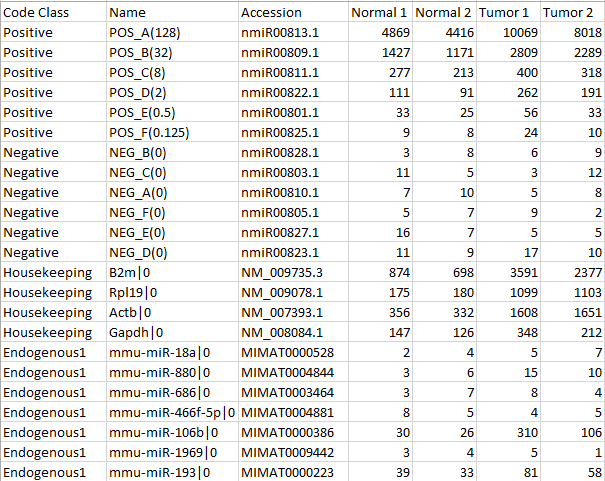
\includegraphics{example.PNG}
  \caption{Example of csv.file pattern}
  \label{example}
\end{figure}




When you created a csv.file, you will specify a variable which 
points on the directory in which your csv.file is located

\begin{Schunk}
\begin{Sinput}
> directory <- "/path/to/your/files/"
\end{Sinput}
\end{Schunk}


However, for demonstration purposes only, the following line of 
code points to the directory for the "Mori.csv" in the 
NanoStringDiff package.

\begin{Schunk}
\begin{Sinput}
> directory <- system.file("extdata", package="NanoStringDiff", mustWork=TRUE)
> path<-paste(directory,"Mori.csv",sep="/")
\end{Sinput}
\end{Schunk}


The phenotype informations of the data should be stored as data frame.
\begin{Schunk}
\begin{Sinput}
> designs=data.frame(group=c("Normal","Normal","Tumor","Tumor"))
> designs
\end{Sinput}
\begin{Soutput}
   group
1 Normal
2 Normal
3  Tumor
4  Tumor
\end{Soutput}
\end{Schunk}


\begin{Schunk}
\begin{Sinput}
> library("NanoStringDiff")
> NanoStringData=createNanoStringSetFromCsv(path,header=TRUE,designs)
\end{Sinput}
\begin{Soutput}
 There are 4 samples imported; 
 There are  618 genes imported with:code.class
 endogenous1  endogenous2 housekeeping     negative     positive      spikein 
         566           33            4            6            6            3 
\end{Soutput}
\begin{Sinput}
> NanoStringData
\end{Sinput}
\begin{Soutput}
NanoStringSet (storageMode: lockedEnvironment)
assayData: 599 features, 4 samples 
  element names: exprs 
protocolData: none
phenoData
  sampleNames: Normal.1 Normal.2 Tumor.1 Tumor.2
  varLabels: group
  varMetadata: labelDescription
featureData: none
experimentData: use 'experimentData(object)'
Annotation:  
\end{Soutput}
\end{Schunk}



\subsection{Create NanoStringSet from matrix}
If you already read your positive control genes, negative control genes, 
housekeeping control genes and endogous into R session separately and 
stored as matrix, then you can use {\tt createNanoStringSet} to create a 
{\tt NanoStringSet} object.


\begin{Schunk}
\begin{Sinput}
> endogenous=matrix(rpois(100,50),25,4)
> colnames(endogenous)=paste("Sample",1:4)
> positive=matrix(rpois(24,c(128,32,8,2,0.5,0.125)*80),6,4)
> colnames(positive)=paste("Sample",1:4)
> negative=matrix(rpois(32,10),8,4)
> colnames(negative)=paste("Sample",1:4)
> housekeeping=matrix(rpois(12,100),3,4)
> colnames(housekeeping)=paste("Sample",1:4)
> designs=data.frame(group=c("Control","Control","Treatment","Treatment"),
+                    gender=c("Male","Female","Female","Male"),
+                    age=c(20,40,39,37))
> NanoStringData1=createNanoStringSet(endogenous,positive,
+                                  negative,housekeeping,designs)
> NanoStringData1
\end{Sinput}
\begin{Soutput}
NanoStringSet (storageMode: lockedEnvironment)
assayData: 25 features, 4 samples 
  element names: exprs 
protocolData: none
phenoData
  sampleNames: Sample 1 Sample 2 Sample 3 Sample 4
  varLabels: group gender age
  varMetadata: labelDescription
featureData: none
experimentData: use 'experimentData(object)'
Annotation:  
\end{Soutput}
\begin{Sinput}
> pData(NanoStringData1)
\end{Sinput}
\begin{Soutput}
             group gender age
Sample 1   Control   Male  20
Sample 2   Control Female  40
Sample 3 Treatment Female  39
Sample 4 Treatment   Male  37
\end{Soutput}
\begin{Sinput}
> head(exprs(NanoStringData1))
\end{Sinput}
\begin{Soutput}
  Sample 1 Sample 2 Sample 3 Sample 4
1       43       52       45       38
2       61       53       52       44
3       49       50       52       54
4       61       45       57       49
5       55       55       53       43
6       60       61       42       54
\end{Soutput}
\end{Schunk}




\section{Differential Expression Analysis for Single Factor Experiment}


For general experiments, once normalization factors obtained using 
{\tt estNormalizationFactors}, given a design matrix and contrast,
we can proceed with testing procedures for determing differential 
expression using the generalized linear model (GLM) likelihood ratio 
test. The testing can be done by using the function {\tt glm.LRT} and
return a list with a component is table including: logFC ,lr, pvalue
and qvalue(adjust p value using the procedure of Benjamini and Hochberg).


\subsection{Two Group Comparisons}

The simplest and most common type of experimental design is two group 
comparison,like treatment group vs control group. As a brief example,
consider a simple situation with control group and  treatment group, 
each with two replicates, and the researcher wants to make comparisons
between them. Here, we still use {\tt NanoSreingData1} we created above
to demonstrate this example.


Make design matrix using {\tt model.matrix}:
\begin{Schunk}
\begin{Sinput}
> pheno=pData(NanoStringData1)
> group=pheno$group
> design.full=model.matrix(~0+group)
> design.full
\end{Sinput}
\begin{Soutput}
  groupControl groupTreatment
1            1              0
2            1              0
3            0              1
4            0              1
attr(,"assign")
[1] 1 1
attr(,"contrasts")
attr(,"contrasts")$group
[1] "contr.treatment"
\end{Soutput}
\end{Schunk}
Note that there is no intercept column in the dasign matrix, each column is 
for each group, since we include {\tt 0+} in the model formula.


If the researcher want compare Treatment to Control, that is Treatment- Control,
the contrast vector is try to the comparison -1*Control+1*Treatment, so the 
contrast is :

\begin{Schunk}
\begin{Sinput}
> contrast=c(-1,1)
\end{Sinput}
\end{Schunk}


Estimate normalization factors and return the same object with positiveFactor,
negativeFactor and housekeepingFactor slots filled or replaced:
\begin{Schunk}
\begin{Sinput}
> NanoStringData1=estNormalizationFactors(NanoStringData1)
> positiveFactor(NanoStringData1)
\end{Sinput}
\begin{Soutput}
 Sample 1  Sample 2  Sample 3  Sample 4 
0.9975706 0.9939514 1.0126318 0.9958463 
\end{Soutput}
\begin{Sinput}
> negativeFactor(NanoStringData1)
\end{Sinput}
\begin{Soutput}
Sample 1 Sample 2 Sample 3 Sample 4 
      10        8        8        9 
\end{Soutput}
\begin{Sinput}
> housekeepingFactor(NanoStringData1)
\end{Sinput}
\begin{Soutput}
 Sample 1  Sample 2  Sample 3  Sample 4 
0.9376834 1.0723536 1.0684187 0.8827223 
\end{Soutput}
\end{Schunk}


Generalize linear model likelihood ratio test:
\begin{Schunk}
\begin{Sinput}
> result=glm.LRT(NanoStringData1,design.full,contrast=contrast)
> head(result$table)
\end{Sinput}
\begin{Soutput}
       logFC         lr    pvalue    qvalue
1 -0.1128736 0.27775294 0.5981778 0.9626035
2 -0.2183201 0.85749477 0.3544407 0.9626035
3  0.1598600 0.38015772 0.5375188 0.9626035
4  0.0483117 0.03288691 0.8560948 0.9626035
5 -0.1883467 0.49894761 0.4799629 0.9626035
6 -0.2115346 1.17415604 0.2785489 0.9626035
\end{Soutput}
\begin{Sinput}
> str(result)
\end{Sinput}
\begin{Soutput}
List of 11
 $ table         :'data.frame':	25 obs. of  4 variables:
  ..$ logFC : num [1:25] -0.1129 -0.2183 0.1599 0.0483 -0.1883 ...
  ..$ lr    : num [1:25] 0.2778 0.8575 0.3802 0.0329 0.4989 ...
  ..$ pvalue: num [1:25] 0.598 0.354 0.538 0.856 0.48 ...
  ..$ qvalue: num [1:25] 0.963 0.963 0.963 0.963 0.963 ...
 $ dispersion    : num [1:25] 0.00618 0.00622 0.00622 0.00623 0.00622 ...
 $ log.dispersion: num [1:25] -5.09 -5.08 -5.08 -5.08 -5.08 ...
 $ design.full   : num [1:4, 1:2] 1 1 0 0 0 0 1 1
  ..- attr(*, "dimnames")=List of 2
  .. ..$ : chr [1:4] "1" "2" "3" "4"
  .. ..$ : chr [1:2] "groupControl" "groupTreatment"
  ..- attr(*, "assign")= int [1:2] 1 1
  ..- attr(*, "contrasts")=List of 1
  .. ..$ group: chr "contr.treatment"
 $ design.reduce : num [1:4, 1] 0.707 0.707 0.707 0.707
  ..- attr(*, "dimnames")=List of 2
  .. ..$ : chr [1:4] "1" "2" "3" "4"
  .. ..$ : NULL
 $ Beta.full     : num [1:25, 1:2] 3.59 3.85 3.7 3.78 3.83 ...
 $ mean.full     : num [1:25, 1:4] 36.4 46.8 40.4 43.8 45.9 ...
  ..- attr(*, "dimnames")=List of 2
  .. ..$ : NULL
  .. ..$ : chr [1:4] "1" "2" "3" "4"
 $ Beta.reduce   : num [1:25] 3.59 3.79 3.76 3.8 3.76 ...
 $ mean.reduce   : num [1:25, 1:4] 36.1 44.1 42.9 44.6 43.1 ...
 $ m0            : num -9.49
 $ sigma         : num 0.1
\end{Soutput}
\end{Schunk}

Note that the text Treatment compare to Control tells you that the estimates 
of logFC is log2(Treatment/Control).










\subsection{Pairwise Comparisons}
Now consider a researcher has three treatment groups say A, B and C, 
and researcher wants to compare each groups like: B compare to A, 
C compare to A, and B compare to C.


First create an object of {\tt NanoStringSet} with pseudo data:
\begin{Schunk}
\begin{Sinput}
> endogenous=matrix(rpois(300,50),25,12)
> colnames(endogenous)=paste("Sample", 1:12)
> colnames(endogenous)=paste("Sample",1:12)
> positive=matrix(rpois(72,c(128,32,8,2,0.5,0.125)*80),6,12)
> negative=matrix(rpois(96,10),8,12)
> housekeeping=matrix(rpois(36,100),3,12)
> designs=data.frame(group=c(rep("A",4),rep("B",4),rep("C",4)),
+                    gender=rep(c("Male","Male","Female","Female"),3),
+                    age=c(20,40,39,37,29,47,23,45,34,65,35,64))
> NanoStringData2=createNanoStringSet(endogenous,positive,
+                                  negative,housekeeping,designs)
> NanoStringData2
\end{Sinput}
\begin{Soutput}
NanoStringSet (storageMode: lockedEnvironment)
assayData: 25 features, 12 samples 
  element names: exprs 
protocolData: none
phenoData
  sampleNames: Sample 1 Sample 2 ... Sample 12 (12 total)
  varLabels: group gender age
  varMetadata: labelDescription
featureData: none
experimentData: use 'experimentData(object)'
Annotation:  
\end{Soutput}
\begin{Sinput}
> pData(NanoStringData2)
\end{Sinput}
\begin{Soutput}
          group gender age
Sample 1      A   Male  20
Sample 2      A   Male  40
Sample 3      A Female  39
Sample 4      A Female  37
Sample 5      B   Male  29
Sample 6      B   Male  47
Sample 7      B Female  23
Sample 8      B Female  45
Sample 9      C   Male  34
Sample 10     C   Male  65
Sample 11     C Female  35
Sample 12     C Female  64
\end{Soutput}
\end{Schunk}



Make design matrix only consider one experimential factor {\tt group}: 
\begin{Schunk}
\begin{Sinput}
> pheno=pData(NanoStringData2)
> group=pheno$group
> design.full=model.matrix(~0+group)
> design.full
\end{Sinput}
\begin{Soutput}
   groupA groupB groupC
1       1      0      0
2       1      0      0
3       1      0      0
4       1      0      0
5       0      1      0
6       0      1      0
7       0      1      0
8       0      1      0
9       0      0      1
10      0      0      1
11      0      0      1
12      0      0      1
attr(,"assign")
[1] 1 1 1
attr(,"contrasts")
attr(,"contrasts")$group
[1] "contr.treatment"
\end{Soutput}
\end{Schunk}

Estimate normalization factors:
\begin{Schunk}
\begin{Sinput}
> NanoStringData2=estNormalizationFactors(NanoStringData2)
\end{Sinput}
\end{Schunk}

B compare to A, the contrast should be (-1,1,0)
\begin{Schunk}
\begin{Sinput}
> result=glm.LRT(NanoStringData2,design.full,contrast=c(-1,1,0))
\end{Sinput}
\end{Schunk}


C compare to A, the contrast should be (-1,0,1)
\begin{Schunk}
\begin{Sinput}
> result=glm.LRT(NanoStringData2,design.full,contrast=c(-1,0,1))
\end{Sinput}
\end{Schunk}


B compare to c, the contrast should be (0,1,-1)
\begin{Schunk}
\begin{Sinput}
> result=glm.LRT(NanoStringData2,design.full,contrast=c(0,1,-1))
\end{Sinput}
\end{Schunk}




The other way to creat a design matrix in R is to include an intercept 
term to represents the base level of the factor. We just omitte 
the {\tt 0+} in the model formula when we create design matrix using 
model.matrix function:

\begin{Schunk}
\begin{Sinput}
> design.full=model.matrix(~group)
> design.full
\end{Sinput}
\begin{Soutput}
   (Intercept) groupB groupC
1            1      0      0
2            1      0      0
3            1      0      0
4            1      0      0
5            1      1      0
6            1      1      0
7            1      1      0
8            1      1      0
9            1      0      1
10           1      0      1
11           1      0      1
12           1      0      1
attr(,"assign")
[1] 0 1 1
attr(,"contrasts")
attr(,"contrasts")$group
[1] "contr.treatment"
\end{Soutput}
\end{Schunk}

In this sitution, the first coefficient measure the log scaler of baseline 
mean expression level in group A, and the second and  third column are now 
relative to the baseline, not represent the mean expression level in 
group B and C. So, if we want to compare B to A, now that is equivalent 
to test the $2^{nd}$ coefficient equal to 0.

\begin{Schunk}
\begin{Sinput}
> result=glm.LRT(NanoStringData2,design.full,Beta=2)
\end{Sinput}
\end{Schunk}

Beta=3 means compare C to A:

\begin{Schunk}
\begin{Sinput}
> result=glm.LRT(NanoStringData2,design.full,Beta=3)
\end{Sinput}
\end{Schunk}






\subsection{Multigroup Comparisons}

NanoStringDiff can do multigroup comparisons, for example if we want 
compare group A to the average of group B and C, 

\begin{Schunk}
\begin{Sinput}
> design.full=model.matrix(~0+group)
> result=glm.LRT(NanoStringData2,design.full,contrast=c(1,-1/2,-1/2))
\end{Sinput}
\end{Schunk}



\section{Differential Expression Analysis for Multifactor Experiment}

In this section, we still use {\tt NanoStringData2} in examples, but the above 
examples all cotnsider single factor {\tt treatment condition} , now we include 
the other experiment factor {\tt gender} to consider multifactor problems.


\subsection{Nested Interactions}
First, we form the design matrix use factors {\tt group} and interaction 
between {\tt group} and {\tt gender}:
\begin{Schunk}
\begin{Sinput}
> design=pData(NanoStringData2)[,c("group","gender")]
> group=design$group
> gender=design$gender
> design.full=model.matrix(~group+group:gender)
> design.full
\end{Sinput}
\begin{Soutput}
   (Intercept) groupB groupC groupA:genderMale groupB:genderMale
1            1      0      0                 1                 0
2            1      0      0                 1                 0
3            1      0      0                 0                 0
4            1      0      0                 0                 0
5            1      1      0                 0                 1
6            1      1      0                 0                 1
7            1      1      0                 0                 0
8            1      1      0                 0                 0
9            1      0      1                 0                 0
10           1      0      1                 0                 0
11           1      0      1                 0                 0
12           1      0      1                 0                 0
   groupC:genderMale
1                  0
2                  0
3                  0
4                  0
5                  0
6                  0
7                  0
8                  0
9                  1
10                 1
11                 0
12                 0
attr(,"assign")
[1] 0 1 1 2 2 2
attr(,"contrasts")
attr(,"contrasts")$group
[1] "contr.treatment"

attr(,"contrasts")$gender
[1] "contr.treatment"
\end{Soutput}
\end{Schunk}

Here, we consider the mean expression level of female in group A as the 
baseline expression level, if we want to test the effect of gender in 
group A, we can use Beta=4,
\begin{Schunk}
\begin{Sinput}
> result=glm.LRT(NanoStringData2,design.full,Beta=4)
\end{Sinput}
\end{Schunk}


Compare treatment group B to A ignore the effect the gender, 
\begin{Schunk}
\begin{Sinput}
> result=glm.LRT(NanoStringData2,design.full,Beta=2)
\end{Sinput}
\end{Schunk}


Consider the interaction effect between gender and group B compare to A:
\begin{Schunk}
\begin{Sinput}
> result=glm.LRT(NanoStringData2,design.full,Beta=c(2,5))
\end{Sinput}
\end{Schunk}


\subsection{All Interactions}
We also can form a design matrix consider all interactions:
\begin{Schunk}
\begin{Sinput}
> design.full=model.matrix(~group+gender+group:gender)
\end{Sinput}
\end{Schunk}

Which is equivalent to:
\begin{Schunk}
\begin{Sinput}
> design.full=model.matrix(~group*gender)
> design.full
\end{Sinput}
\begin{Soutput}
   (Intercept) groupB groupC genderMale groupB:genderMale groupC:genderMale
1            1      0      0          1                 0                 0
2            1      0      0          1                 0                 0
3            1      0      0          0                 0                 0
4            1      0      0          0                 0                 0
5            1      1      0          1                 1                 0
6            1      1      0          1                 1                 0
7            1      1      0          0                 0                 0
8            1      1      0          0                 0                 0
9            1      0      1          1                 0                 1
10           1      0      1          1                 0                 1
11           1      0      1          0                 0                 0
12           1      0      1          0                 0                 0
attr(,"assign")
[1] 0 1 1 2 3 3
attr(,"contrasts")
attr(,"contrasts")$group
[1] "contr.treatment"

attr(,"contrasts")$gender
[1] "contr.treatment"
\end{Soutput}
\end{Schunk}


Test the gender effect in Treatment group B:
\begin{Schunk}
\begin{Sinput}
> result=glm.LRT(NanoStringData2,design.full,Beta=4:5)
\end{Sinput}
\end{Schunk}



\section{Session Info}

\begin{Schunk}
\begin{Sinput}
> toLatex(sessionInfo())
\end{Sinput}
\begin{itemize}\raggedright
  \item R version 3.4.1 (2017-06-30), \verb|x86_64-apple-darwin15.6.0|
  \item Locale: \verb|en_US.UTF-8/en_US.UTF-8/en_US.UTF-8/C/en_US.UTF-8/en_US.UTF-8|
  \item Running under: \verb|OS X El Capitan 10.11.6|
  \item Matrix products: default
  \item BLAS: \verb|/Library/Frameworks/R.framework/Versions/3.4/Resources/lib/libRblas.0.dylib|
  \item LAPACK: \verb|/Library/Frameworks/R.framework/Versions/3.4/Resources/lib/libRlapack.dylib|
  \item Base packages: base, datasets, graphics, grDevices, methods,
    parallel, stats, utils
  \item Other packages: Biobase~2.38.0, BiocGenerics~0.24.0,
    NanoStringDiff~1.8.1
  \item Loaded via a namespace (and not attached): compiler~3.4.1,
    matrixStats~0.53.0, Rcpp~0.12.15, tools~3.4.1
\end{itemize}\end{Schunk}

\bibliography{reference}


\end{document}
